\documentclass[1p]{elsarticle_modified}
%\bibliographystyle{elsarticle-num}

%\usepackage[colorlinks]{hyperref}
%\usepackage{abbrmath_seonhwa} %\Abb, \Ascr, \Acal ,\Abf, \Afrak
\usepackage{amsfonts}
\usepackage{amssymb}
\usepackage{amsmath}
\usepackage{amsthm}
\usepackage{scalefnt}
\usepackage{amsbsy}
\usepackage{kotex}
\usepackage{caption}
\usepackage{subfig}
\usepackage{color}
\usepackage{graphicx}
\usepackage{xcolor} %% white, black, red, green, blue, cyan, magenta, yellow
\usepackage{float}
\usepackage{setspace}
\usepackage{hyperref}

\usepackage{tikz}
\usetikzlibrary{arrows}

\usepackage{multirow}
\usepackage{array} % fixed length table
\usepackage{hhline}

%%%%%%%%%%%%%%%%%%%%%
\makeatletter
\renewcommand*\env@matrix[1][\arraystretch]{%
	\edef\arraystretch{#1}%
	\hskip -\arraycolsep
	\let\@ifnextchar\new@ifnextchar
	\array{*\c@MaxMatrixCols c}}
\makeatother %https://tex.stackexchange.com/questions/14071/how-can-i-increase-the-line-spacing-in-a-matrix
%%%%%%%%%%%%%%%

\usepackage[normalem]{ulem}

\newcommand{\msout}[1]{\ifmmode\text{\sout{\ensuremath{#1}}}\else\sout{#1}\fi}
%SOURCE: \msout is \stkout macro in https://tex.stackexchange.com/questions/20609/strikeout-in-math-mode

\newcommand{\cancel}[1]{
	\ifmmode
	{\color{red}\msout{#1}}
	\else
	{\color{red}\sout{#1}}
	\fi
}

\newcommand{\add}[1]{
	{\color{blue}\uwave{#1}}
}

\newcommand{\replace}[2]{
	\ifmmode
	{\color{red}\msout{#1}}{\color{blue}\uwave{#2}}
	\else
	{\color{red}\sout{#1}}{\color{blue}\uwave{#2}}
	\fi
}

\newcommand{\Sol}{\mathcal{S}} %segment
\newcommand{\D}{D} %diagram
\newcommand{\A}{\mathcal{A}} %arc


%%%%%%%%%%%%%%%%%%%%%%%%%%%%%5 test

\def\sl{\operatorname{\textup{SL}}(2,\Cbb)}
\def\psl{\operatorname{\textup{PSL}}(2,\Cbb)}
\def\quan{\mkern 1mu \triangleright \mkern 1mu}

\theoremstyle{definition}
\newtheorem{thm}{Theorem}[section]
\newtheorem{prop}[thm]{Proposition}
\newtheorem{lem}[thm]{Lemma}
\newtheorem{ques}[thm]{Question}
\newtheorem{cor}[thm]{Corollary}
\newtheorem{defn}[thm]{Definition}
\newtheorem{exam}[thm]{Example}
\newtheorem{rmk}[thm]{Remark}
\newtheorem{alg}[thm]{Algorithm}

\newcommand{\I}{\sqrt{-1}}
\begin{document}

%\begin{frontmatter}
%
%\title{Boundary parabolic representations of knots up to 8 crossings}
%
%%% Group authors per affiliation:
%\author{Yunhi Cho} 
%\address{Department of Mathematics, University of Seoul, Seoul, Korea}
%\ead{yhcho@uos.ac.kr}
%
%
%\author{Seonhwa Kim} %\fnref{s_kim}}
%\address{Center for Geometry and Physics, Institute for Basic Science, Pohang, 37673, Korea}
%\ead{ryeona17@ibs.re.kr}
%
%\author{Hyuk Kim}
%\address{Department of Mathematical Sciences, Seoul National University, Seoul 08826, Korea}
%\ead{hyukkim@snu.ac.kr}
%
%\author{Seokbeom Yoon}
%\address{Department of Mathematical Sciences, Seoul National University, Seoul, 08826,  Korea}
%\ead{sbyoon15@snu.ac.kr}
%
%\begin{abstract}
%We find all boundary parabolic representation of knots up to 8 crossings.
%
%\end{abstract}
%\begin{keyword}
%    \MSC[2010] 57M25 
%\end{keyword}
%
%\end{frontmatter}

%\linenumbers
%\tableofcontents
%
\newcommand\colored[1]{\textcolor{white}{\rule[-0.35ex]{0.8em}{1.4ex}}\kern-0.8em\color{red} #1}%
%\newcommand\colored[1]{\textcolor{white}{ #1}\kern-2.17ex	\textcolor{white}{ #1}\kern-1.81ex	\textcolor{white}{ #1}\kern-2.15ex\color{red}#1	}

{\Large $\underline{12a_{0258}~(K12a_{0258})}$}

\setlength{\tabcolsep}{10pt}
\renewcommand{\arraystretch}{1.6}
\vspace{1cm}\begin{tabular}{m{100pt}>{\centering\arraybackslash}m{274pt}}
\multirow{5}{120pt}{
	\centering
	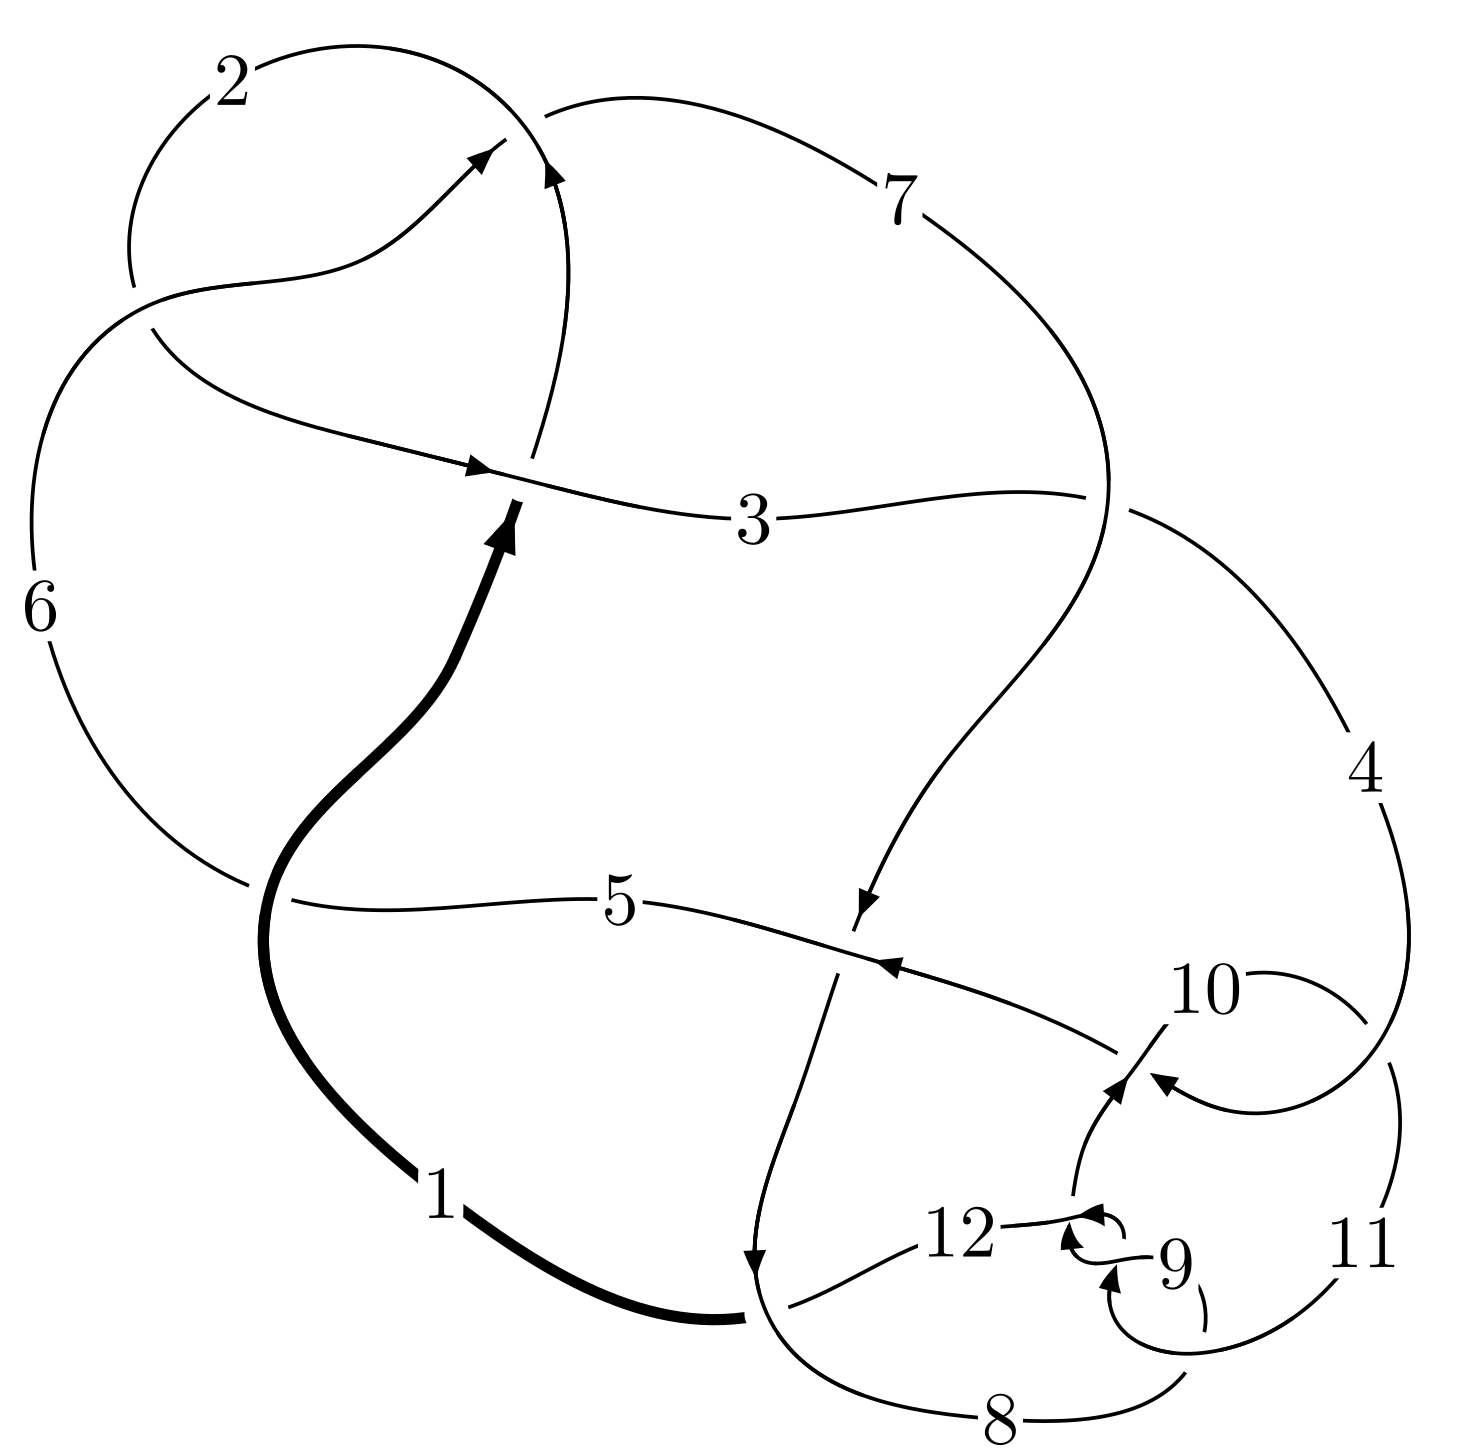
\includegraphics[width=112pt]{../../../GIT/diagram.site/Diagrams/png/1059_12a_0258.png}\\
\ \ \ A knot diagram\footnotemark}&
\allowdisplaybreaks
\textbf{Linearized knot diagam} \\
\cline{2-2}
 &
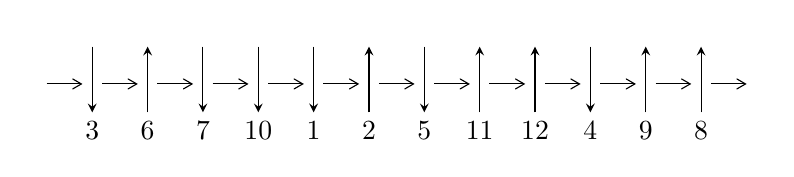
\begin{tikzpicture}[x=20pt, y=17pt]
	% nodes
	\node (C0) at (0, 0) {};
	\node (C1) at (1, 0) {};
	\node (C1U) at (1, +1) {};
	\node (C1D) at (1, -1) {3};

	\node (C2) at (2, 0) {};
	\node (C2U) at (2, +1) {};
	\node (C2D) at (2, -1) {6};

	\node (C3) at (3, 0) {};
	\node (C3U) at (3, +1) {};
	\node (C3D) at (3, -1) {7};

	\node (C4) at (4, 0) {};
	\node (C4U) at (4, +1) {};
	\node (C4D) at (4, -1) {10};

	\node (C5) at (5, 0) {};
	\node (C5U) at (5, +1) {};
	\node (C5D) at (5, -1) {1};

	\node (C6) at (6, 0) {};
	\node (C6U) at (6, +1) {};
	\node (C6D) at (6, -1) {2};

	\node (C7) at (7, 0) {};
	\node (C7U) at (7, +1) {};
	\node (C7D) at (7, -1) {5};

	\node (C8) at (8, 0) {};
	\node (C8U) at (8, +1) {};
	\node (C8D) at (8, -1) {11};

	\node (C9) at (9, 0) {};
	\node (C9U) at (9, +1) {};
	\node (C9D) at (9, -1) {12};

	\node (C10) at (10, 0) {};
	\node (C10U) at (10, +1) {};
	\node (C10D) at (10, -1) {4};

	\node (C11) at (11, 0) {};
	\node (C11U) at (11, +1) {};
	\node (C11D) at (11, -1) {9};

	\node (C12) at (12, 0) {};
	\node (C12U) at (12, +1) {};
	\node (C12D) at (12, -1) {8};
	\node (C13) at (13, 0) {};

	% arrows
	\draw[->,>={angle 60}]
	(C0) edge (C1) (C1) edge (C2) (C2) edge (C3) (C3) edge (C4) (C4) edge (C5) (C5) edge (C6) (C6) edge (C7) (C7) edge (C8) (C8) edge (C9) (C9) edge (C10) (C10) edge (C11) (C11) edge (C12) (C12) edge (C13) ;	\draw[->,>=stealth]
	(C1U) edge (C1D) (C2D) edge (C2U) (C3U) edge (C3D) (C4U) edge (C4D) (C5U) edge (C5D) (C6D) edge (C6U) (C7U) edge (C7D) (C8D) edge (C8U) (C9D) edge (C9U) (C10U) edge (C10D) (C11D) edge (C11U) (C12D) edge (C12U) ;
	\end{tikzpicture} \\
\hhline{~~} \\& 
\textbf{Solving Sequence} \\ \cline{2-2} 
 &
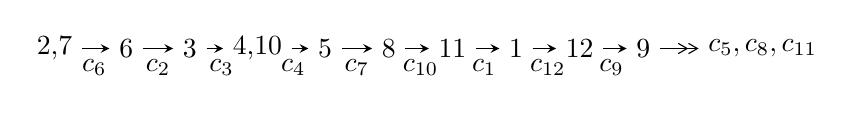
\begin{tikzpicture}[x=23pt, y=7pt]
	% node
	\node (A0) at (-1/8, 0) {2,7};
	\node (A1) at (1, 0) {6};
	\node (A2) at (2, 0) {3};
	\node (A3) at (49/16, 0) {4,10};
	\node (A4) at (33/8, 0) {5};
	\node (A5) at (41/8, 0) {8};
	\node (A6) at (49/8, 0) {11};
	\node (A7) at (57/8, 0) {1};
	\node (A8) at (65/8, 0) {12};
	\node (A9) at (73/8, 0) {9};
	\node (C1) at (1/2, -1) {$c_{6}$};
	\node (C2) at (3/2, -1) {$c_{2}$};
	\node (C3) at (5/2, -1) {$c_{3}$};
	\node (C4) at (29/8, -1) {$c_{4}$};
	\node (C5) at (37/8, -1) {$c_{7}$};
	\node (C6) at (45/8, -1) {$c_{10}$};
	\node (C7) at (53/8, -1) {$c_{1}$};
	\node (C8) at (61/8, -1) {$c_{12}$};
	\node (C9) at (69/8, -1) {$c_{9}$};
	\node (A10) at (11, 0) {$c_{5},c_{8},c_{11}$};

	% edge
	\draw[->,>=stealth]	
	(A0) edge (A1) (A1) edge (A2) (A2) edge (A3) (A3) edge (A4) (A4) edge (A5) (A5) edge (A6) (A6) edge (A7) (A7) edge (A8) (A8) edge (A9) ;
	\draw[->>,>={angle 60}]	
	(A9) edge (A10);
\end{tikzpicture} \\ 

\end{tabular} \\

\footnotetext{
The image of knot diagram is generated by the software ``\textbf{Draw programme}" developed by Andrew Bartholomew(\url{http://www.layer8.co.uk/maths/draw/index.htm\#Running-draw}), where we modified some parts for our purpose(\url{https://github.com/CATsTAILs/LinksPainter}).
}\phantom \\ \newline 
\centering \textbf{Ideals for irreducible components\footnotemark of $X_{\text{par}}$} 
 
\begin{align*}
I^u_{1}&=\langle 
- u^{87}+u^{86}+\cdots+b+u,\;2 u^{87}-2 u^{86}+\cdots+a+1,\;u^{89}-2 u^{88}+\cdots-3 u+1\rangle \\
I^u_{2}&=\langle 
b+1,\;- u^3- u^2+a- u-1,\;u^5+u^4+2 u^3+u^2+u+1\rangle \\
\\
\end{align*}
\raggedright * 2 irreducible components of $\dim_{\mathbb{C}}=0$, with total 94 representations.\\
\footnotetext{All coefficients of polynomials are rational numbers. But the coefficients are sometimes approximated in decimal forms when there is not enough margin.}
\newpage
\renewcommand{\arraystretch}{1}
\centering \section*{I. $I^u_{1}= \langle - u^{87}+u^{86}+\cdots+b+u,\;2 u^{87}-2 u^{86}+\cdots+a+1,\;u^{89}-2 u^{88}+\cdots-3 u+1 \rangle$}
\flushleft \textbf{(i) Arc colorings}\\
\begin{tabular}{m{7pt} m{180pt} m{7pt} m{180pt} }
\flushright $a_{2}=$&$\begin{pmatrix}0\\u\end{pmatrix}$ \\
\flushright $a_{7}=$&$\begin{pmatrix}1\\0\end{pmatrix}$ \\
\flushright $a_{6}=$&$\begin{pmatrix}1\\u^2\end{pmatrix}$ \\
\flushright $a_{3}=$&$\begin{pmatrix}u\\u^3+u\end{pmatrix}$ \\
\flushright $a_{4}=$&$\begin{pmatrix}- u^3\\u^3+u\end{pmatrix}$ \\
\flushright $a_{10}=$&$\begin{pmatrix}-2 u^{87}+2 u^{86}+\cdots+3 u-1\\u^{87}- u^{86}+\cdots+u^2- u\end{pmatrix}$ \\
\flushright $a_{5}=$&$\begin{pmatrix}- u^6- u^4+1\\- u^8-2 u^6-2 u^4\end{pmatrix}$ \\
\flushright $a_{8}=$&$\begin{pmatrix}u^{14}+3 u^{12}+4 u^{10}+u^8-2 u^6-2 u^4+1\\u^{16}+4 u^{14}+8 u^{12}+8 u^{10}+4 u^8\end{pmatrix}$ \\
\flushright $a_{11}=$&$\begin{pmatrix}- u^{84}+u^{83}+\cdots- u^3+2 u^2\\- u^{86}+u^{85}+\cdots+u^5- u^2\end{pmatrix}$ \\
\flushright $a_{1}=$&$\begin{pmatrix}u^3\\u^5+u^3+u\end{pmatrix}$ \\
\flushright $a_{12}=$&$\begin{pmatrix}u^{25}+6 u^{23}+\cdots+3 u^5- u\\u^{27}+7 u^{25}+\cdots+u^3+u\end{pmatrix}$ \\
\flushright $a_{9}=$&$\begin{pmatrix}- u^{87}+u^{86}+\cdots- u^3+u\\u^{87}- u^{86}+\cdots+4 u^5- u^4\end{pmatrix}$\\&\end{tabular}
\flushleft \textbf{(ii) Obstruction class $= -1$}\\~\\
\flushleft \textbf{(iii) Cusp Shapes $= -4 u^{88}+13 u^{87}+\cdots-20 u+9$}\\~\\
\newpage\renewcommand{\arraystretch}{1}
\flushleft \textbf{(iv) u-Polynomials at the component}\newline \\
\begin{tabular}{m{50pt}|m{274pt}}
Crossings & \hspace{64pt}u-Polynomials at each crossing \\
\hline $$\begin{aligned}c_{1}\end{aligned}$$&$\begin{aligned}
&u^{89}+48 u^{88}+\cdots+u-1
\end{aligned}$\\
\hline $$\begin{aligned}c_{2},c_{6}\end{aligned}$$&$\begin{aligned}
&u^{89}-2 u^{88}+\cdots-3 u+1
\end{aligned}$\\
\hline $$\begin{aligned}c_{3},c_{5}\end{aligned}$$&$\begin{aligned}
&u^{89}+2 u^{88}+\cdots+9 u+1
\end{aligned}$\\
\hline $$\begin{aligned}c_{4},c_{10}\end{aligned}$$&$\begin{aligned}
&u^{89}- u^{88}+\cdots+120 u^2+32
\end{aligned}$\\
\hline $$\begin{aligned}c_{7}\end{aligned}$$&$\begin{aligned}
&u^{89}-12 u^{88}+\cdots-3133 u+277
\end{aligned}$\\
\hline $$\begin{aligned}c_{8},c_{9},c_{11}\end{aligned}$$&$\begin{aligned}
&u^{89}+6 u^{88}+\cdots+3 u+1
\end{aligned}$\\
\hline $$\begin{aligned}c_{12}\end{aligned}$$&$\begin{aligned}
&u^{89}-33 u^{88}+\cdots-7680 u+1024
\end{aligned}$\\
\hline
\end{tabular}\\~\\
\newpage\renewcommand{\arraystretch}{1}
\flushleft \textbf{(v) Riley Polynomials at the component}\newline \\
\begin{tabular}{m{50pt}|m{274pt}}
Crossings & \hspace{64pt}Riley Polynomials at each crossing \\
\hline $$\begin{aligned}c_{1}\end{aligned}$$&$\begin{aligned}
&y^{89}-12 y^{88}+\cdots+9 y-1
\end{aligned}$\\
\hline $$\begin{aligned}c_{2},c_{6}\end{aligned}$$&$\begin{aligned}
&y^{89}+48 y^{88}+\cdots+y-1
\end{aligned}$\\
\hline $$\begin{aligned}c_{3},c_{5}\end{aligned}$$&$\begin{aligned}
&y^{89}-72 y^{88}+\cdots+145 y-1
\end{aligned}$\\
\hline $$\begin{aligned}c_{4},c_{10}\end{aligned}$$&$\begin{aligned}
&y^{89}+33 y^{88}+\cdots-7680 y-1024
\end{aligned}$\\
\hline $$\begin{aligned}c_{7}\end{aligned}$$&$\begin{aligned}
&y^{89}-12 y^{88}+\cdots-1273175 y-76729
\end{aligned}$\\
\hline $$\begin{aligned}c_{8},c_{9},c_{11}\end{aligned}$$&$\begin{aligned}
&y^{89}-76 y^{88}+\cdots-21 y-1
\end{aligned}$\\
\hline $$\begin{aligned}c_{12}\end{aligned}$$&$\begin{aligned}
&y^{89}+37 y^{88}+\cdots-14024704 y-1048576
\end{aligned}$\\
\hline
\end{tabular}\\~\\
\newpage\flushleft \textbf{(vi) Complex Volumes and Cusp Shapes}
$$\begin{array}{c|c|c}  
\text{Solutions to }I^u_{1}& \I (\text{vol} + \sqrt{-1}CS) & \text{Cusp shape}\\
 \hline 
\begin{aligned}
u &= \phantom{-}0.517663 + 0.853057 I \\
a &= \phantom{-}0.063168 + 1.010150 I \\
b &= \phantom{-}0.0075337 + 0.0380861 I\end{aligned}
 & \phantom{-}3.01994 + 4.86569 I & \phantom{-0.000000 } 0 \\ \hline\begin{aligned}
u &= \phantom{-}0.517663 - 0.853057 I \\
a &= \phantom{-}0.063168 - 1.010150 I \\
b &= \phantom{-}0.0075337 - 0.0380861 I\end{aligned}
 & \phantom{-}3.01994 - 4.86569 I & \phantom{-0.000000 } 0 \\ \hline\begin{aligned}
u &= \phantom{-}0.448323 + 0.897280 I \\
a &= \phantom{-}0.215044 - 0.933260 I \\
b &= -0.0257289 + 0.0936950 I\end{aligned}
 & -1.14920 + 2.08020 I & \phantom{-0.000000 } 0 \\ \hline\begin{aligned}
u &= \phantom{-}0.448323 - 0.897280 I \\
a &= \phantom{-}0.215044 + 0.933260 I \\
b &= -0.0257289 - 0.0936950 I\end{aligned}
 & -1.14920 - 2.08020 I & \phantom{-0.000000 } 0 \\ \hline\begin{aligned}
u &= -0.527593 + 0.875296 I \\
a &= \phantom{-}0.04378 + 1.59082 I \\
b &= \phantom{-}1.91935 - 0.02195 I\end{aligned}
 & \phantom{-}0.04402 - 6.76781 I & \phantom{-0.000000 } 0 \\ \hline\begin{aligned}
u &= -0.527593 - 0.875296 I \\
a &= \phantom{-}0.04378 - 1.59082 I \\
b &= \phantom{-}1.91935 + 0.02195 I\end{aligned}
 & \phantom{-}0.04402 + 6.76781 I & \phantom{-0.000000 } 0 \\ \hline\begin{aligned}
u &= \phantom{-}0.045374 + 1.026840 I \\
a &= -1.396320 + 0.027423 I \\
b &= \phantom{-}0.762961 + 0.584535 I\end{aligned}
 & -3.82045 + 2.55031 I & \phantom{-0.000000 } 0 \\ \hline\begin{aligned}
u &= \phantom{-}0.045374 - 1.026840 I \\
a &= -1.396320 - 0.027423 I \\
b &= \phantom{-}0.762961 - 0.584535 I\end{aligned}
 & -3.82045 - 2.55031 I & \phantom{-0.000000 } 0 \\ \hline\begin{aligned}
u &= -0.036660 + 0.970796 I \\
a &= \phantom{-}1.45328 + 0.01748 I \\
b &= -0.651637 - 0.810834 I\end{aligned}
 & -0.611498 - 1.156220 I & \phantom{-0.000000 } 0 \\ \hline\begin{aligned}
u &= -0.036660 - 0.970796 I \\
a &= \phantom{-}1.45328 - 0.01748 I \\
b &= -0.651637 + 0.810834 I\end{aligned}
 & -0.611498 + 1.156220 I & \phantom{-0.000000 } 0\\
 \hline 
 \end{array}$$\newpage$$\begin{array}{c|c|c}  
\text{Solutions to }I^u_{1}& \I (\text{vol} + \sqrt{-1}CS) & \text{Cusp shape}\\
 \hline 
\begin{aligned}
u &= -0.487998 + 0.832637 I \\
a &= -0.15557 - 1.88628 I \\
b &= -2.07823 + 0.10861 I\end{aligned}
 & \phantom{-}2.18808 - 2.44281 I & \phantom{-0.000000 } 0 \\ \hline\begin{aligned}
u &= -0.487998 - 0.832637 I \\
a &= -0.15557 + 1.88628 I \\
b &= -2.07823 - 0.10861 I\end{aligned}
 & \phantom{-}2.18808 + 2.44281 I & \phantom{-0.000000 } 0 \\ \hline\begin{aligned}
u &= -0.558903 + 0.882043 I \\
a &= -0.09933 - 1.47746 I \\
b &= -1.86773 + 0.05365 I\end{aligned}
 & \phantom{-}5.18287 - 10.77750 I & \phantom{-0.000000 } 0 \\ \hline\begin{aligned}
u &= -0.558903 - 0.882043 I \\
a &= -0.09933 + 1.47746 I \\
b &= -1.86773 - 0.05365 I\end{aligned}
 & \phantom{-}5.18287 + 10.77750 I & \phantom{-0.000000 } 0 \\ \hline\begin{aligned}
u &= -0.570217 + 0.765010 I \\
a &= \phantom{-}0.46901 + 1.53140 I \\
b &= \phantom{-}1.82570 - 0.18189 I\end{aligned}
 & \phantom{-}9.81950 - 2.26683 I & \phantom{-}9.08032 + 0. I\phantom{ +0.000000I} \\ \hline\begin{aligned}
u &= -0.570217 - 0.765010 I \\
a &= \phantom{-}0.46901 - 1.53140 I \\
b &= \phantom{-}1.82570 + 0.18189 I\end{aligned}
 & \phantom{-}9.81950 + 2.26683 I & \phantom{-}9.08032 + 0. I\phantom{ +0.000000I} \\ \hline\begin{aligned}
u &= \phantom{-}0.083364 + 1.074910 I \\
a &= \phantom{-}1.42919 - 0.06261 I \\
b &= -0.891162 - 0.475610 I\end{aligned}
 & \phantom{-}0.70579 + 6.29860 I & \phantom{-0.000000 } 0 \\ \hline\begin{aligned}
u &= \phantom{-}0.083364 - 1.074910 I \\
a &= \phantom{-}1.42919 + 0.06261 I \\
b &= -0.891162 + 0.475610 I\end{aligned}
 & \phantom{-}0.70579 - 6.29860 I & \phantom{-0.000000 } 0 \\ \hline\begin{aligned}
u &= \phantom{-}0.479594 + 1.025290 I \\
a &= -0.47420 + 1.59768 I \\
b &= -0.230291 - 0.441844 I\end{aligned}
 & \phantom{-}3.30132 - 0.46498 I & \phantom{-0.000000 } 0 \\ \hline\begin{aligned}
u &= \phantom{-}0.479594 - 1.025290 I \\
a &= -0.47420 - 1.59768 I \\
b &= -0.230291 + 0.441844 I\end{aligned}
 & \phantom{-}3.30132 + 0.46498 I & \phantom{-0.000000 } 0\\
 \hline 
 \end{array}$$\newpage$$\begin{array}{c|c|c}  
\text{Solutions to }I^u_{1}& \I (\text{vol} + \sqrt{-1}CS) & \text{Cusp shape}\\
 \hline 
\begin{aligned}
u &= -0.472021 + 0.710727 I \\
a &= -0.85417 - 1.74292 I \\
b &= -1.77547 + 0.50967 I\end{aligned}
 & \phantom{-}2.55068 - 1.56908 I & \phantom{-}7.62928 + 3.25616 I \\ \hline\begin{aligned}
u &= -0.472021 - 0.710727 I \\
a &= -0.85417 + 1.74292 I \\
b &= -1.77547 - 0.50967 I\end{aligned}
 & \phantom{-}2.55068 + 1.56908 I & \phantom{-}7.62928 - 3.25616 I \\ \hline\begin{aligned}
u &= -0.586040 + 0.618786 I \\
a &= -0.73818 - 1.29420 I \\
b &= -1.52005 + 0.15803 I\end{aligned}
 & \phantom{-}5.92566 + 6.23892 I & \phantom{-}6.49865 - 3.39583 I \\ \hline\begin{aligned}
u &= -0.586040 - 0.618786 I \\
a &= -0.73818 + 1.29420 I \\
b &= -1.52005 - 0.15803 I\end{aligned}
 & \phantom{-}5.92566 - 6.23892 I & \phantom{-}6.49865 + 3.39583 I \\ \hline\begin{aligned}
u &= \phantom{-}0.318408 + 1.117220 I \\
a &= -1.78251 + 0.77997 I \\
b &= \phantom{-}0.924881 - 0.530367 I\end{aligned}
 & \phantom{-}3.57675 - 0.11414 I & \phantom{-0.000000 } 0 \\ \hline\begin{aligned}
u &= \phantom{-}0.318408 - 1.117220 I \\
a &= -1.78251 - 0.77997 I \\
b &= \phantom{-}0.924881 + 0.530367 I\end{aligned}
 & \phantom{-}3.57675 + 0.11414 I & \phantom{-0.000000 } 0 \\ \hline\begin{aligned}
u &= \phantom{-}0.821589 + 0.144980 I \\
a &= \phantom{-}0.196200 - 0.728902 I \\
b &= -2.16374 + 0.76355 I\end{aligned}
 & \phantom{-}1.51929 - 11.34500 I & \phantom{-}2.72775 + 7.03467 I \\ \hline\begin{aligned}
u &= \phantom{-}0.821589 - 0.144980 I \\
a &= \phantom{-}0.196200 + 0.728902 I \\
b &= -2.16374 - 0.76355 I\end{aligned}
 & \phantom{-}1.51929 + 11.34500 I & \phantom{-}2.72775 - 7.03467 I \\ \hline\begin{aligned}
u &= \phantom{-}0.505613 + 0.657363 I \\
a &= -0.353180 - 0.878368 I \\
b &= -0.302339 + 0.026911 I\end{aligned}
 & \phantom{-}3.57630 - 0.65503 I & \phantom{-}5.49721 - 0.67822 I \\ \hline\begin{aligned}
u &= \phantom{-}0.505613 - 0.657363 I \\
a &= -0.353180 + 0.878368 I \\
b &= -0.302339 - 0.026911 I\end{aligned}
 & \phantom{-}3.57630 + 0.65503 I & \phantom{-}5.49721 + 0.67822 I\\
 \hline 
 \end{array}$$\newpage$$\begin{array}{c|c|c}  
\text{Solutions to }I^u_{1}& \I (\text{vol} + \sqrt{-1}CS) & \text{Cusp shape}\\
 \hline 
\begin{aligned}
u &= -0.824465 + 0.058272 I \\
a &= \phantom{-}0.173870 + 0.454318 I \\
b &= \phantom{-}0.247863 + 0.493086 I\end{aligned}
 & -0.95526 - 1.82340 I & \phantom{-}2.00883 + 3.90836 I \\ \hline\begin{aligned}
u &= -0.824465 - 0.058272 I \\
a &= \phantom{-}0.173870 - 0.454318 I \\
b &= \phantom{-}0.247863 - 0.493086 I\end{aligned}
 & -0.95526 + 1.82340 I & \phantom{-}2.00883 - 3.90836 I \\ \hline\begin{aligned}
u &= \phantom{-}0.807857 + 0.130335 I \\
a &= -0.257591 + 0.772643 I \\
b &= \phantom{-}2.20223 - 0.92168 I\end{aligned}
 & -3.42851 - 7.01835 I & -1.34084 + 5.91260 I \\ \hline\begin{aligned}
u &= \phantom{-}0.807857 - 0.130335 I \\
a &= -0.257591 - 0.772643 I \\
b &= \phantom{-}2.20223 + 0.92168 I\end{aligned}
 & -3.42851 + 7.01835 I & -1.34084 - 5.91260 I \\ \hline\begin{aligned}
u &= \phantom{-}0.302386 + 0.751486 I \\
a &= \phantom{-}0.521010 + 0.407084 I \\
b &= \phantom{-}0.034676 - 0.191296 I\end{aligned}
 & -0.337993 + 1.231430 I & -4.05082 - 5.12187 I \\ \hline\begin{aligned}
u &= \phantom{-}0.302386 - 0.751486 I \\
a &= \phantom{-}0.521010 - 0.407084 I \\
b &= \phantom{-}0.034676 + 0.191296 I\end{aligned}
 & -0.337993 - 1.231430 I & -4.05082 + 5.12187 I \\ \hline\begin{aligned}
u &= -0.527637 + 0.613852 I \\
a &= \phantom{-}0.86201 + 1.35059 I \\
b &= \phantom{-}1.47210 - 0.29714 I\end{aligned}
 & \phantom{-}0.77238 + 2.47093 I & \phantom{-}2.67534 - 2.90980 I \\ \hline\begin{aligned}
u &= -0.527637 - 0.613852 I \\
a &= \phantom{-}0.86201 - 1.35059 I \\
b &= \phantom{-}1.47210 + 0.29714 I\end{aligned}
 & \phantom{-}0.77238 - 2.47093 I & \phantom{-}2.67534 + 2.90980 I \\ \hline\begin{aligned}
u &= -0.800030 + 0.093267 I \\
a &= -0.289719 - 0.456598 I \\
b &= -0.393360 - 0.440336 I\end{aligned}
 & -4.50871 + 1.54087 I & -3.93955 - 0.53955 I \\ \hline\begin{aligned}
u &= -0.800030 - 0.093267 I \\
a &= -0.289719 + 0.456598 I \\
b &= -0.393360 + 0.440336 I\end{aligned}
 & -4.50871 - 1.54087 I & -3.93955 + 0.53955 I\\
 \hline 
 \end{array}$$\newpage$$\begin{array}{c|c|c}  
\text{Solutions to }I^u_{1}& \I (\text{vol} + \sqrt{-1}CS) & \text{Cusp shape}\\
 \hline 
\begin{aligned}
u &= -0.792991 + 0.129489 I \\
a &= \phantom{-}0.362212 + 0.510270 I \\
b &= \phantom{-}0.508182 + 0.450575 I\end{aligned}
 & -0.18794 + 5.08047 I & \phantom{-}1.48224 - 3.61614 I \\ \hline\begin{aligned}
u &= -0.792991 - 0.129489 I \\
a &= \phantom{-}0.362212 - 0.510270 I \\
b &= \phantom{-}0.508182 - 0.450575 I\end{aligned}
 & -0.18794 - 5.08047 I & \phantom{-}1.48224 + 3.61614 I \\ \hline\begin{aligned}
u &= \phantom{-}0.780635 + 0.114182 I \\
a &= \phantom{-}0.321976 - 0.894632 I \\
b &= -2.15166 + 1.23701 I\end{aligned}
 & -0.76764 - 2.40112 I & \phantom{-}1.86669 + 2.82981 I \\ \hline\begin{aligned}
u &= \phantom{-}0.780635 - 0.114182 I \\
a &= \phantom{-}0.321976 + 0.894632 I \\
b &= -2.15166 - 1.23701 I\end{aligned}
 & -0.76764 + 2.40112 I & \phantom{-}1.86669 - 2.82981 I \\ \hline\begin{aligned}
u &= \phantom{-}0.435439 + 1.137790 I \\
a &= \phantom{-}1.87502 - 2.52725 I \\
b &= -0.13112 + 1.68520 I\end{aligned}
 & -2.30698 + 1.91588 I & \phantom{-0.000000 } 0 \\ \hline\begin{aligned}
u &= \phantom{-}0.435439 - 1.137790 I \\
a &= \phantom{-}1.87502 + 2.52725 I \\
b &= -0.13112 - 1.68520 I\end{aligned}
 & -2.30698 - 1.91588 I & \phantom{-0.000000 } 0 \\ \hline\begin{aligned}
u &= -0.462237 + 1.138890 I \\
a &= \phantom{-}0.265455 - 0.514615 I \\
b &= -0.847571 - 0.105524 I\end{aligned}
 & -0.25321 - 3.93959 I & \phantom{-0.000000 } 0 \\ \hline\begin{aligned}
u &= -0.462237 - 1.138890 I \\
a &= \phantom{-}0.265455 + 0.514615 I \\
b &= -0.847571 + 0.105524 I\end{aligned}
 & -0.25321 + 3.93959 I & \phantom{-0.000000 } 0 \\ \hline\begin{aligned}
u &= \phantom{-}0.730068 + 0.216859 I \\
a &= \phantom{-}0.017747 + 0.955576 I \\
b &= \phantom{-}1.41229 - 0.75798 I\end{aligned}
 & \phantom{-}7.51403 - 3.34035 I & \phantom{-}7.60444 + 3.00182 I \\ \hline\begin{aligned}
u &= \phantom{-}0.730068 - 0.216859 I \\
a &= \phantom{-}0.017747 - 0.955576 I \\
b &= \phantom{-}1.41229 + 0.75798 I\end{aligned}
 & \phantom{-}7.51403 + 3.34035 I & \phantom{-}7.60444 - 3.00182 I\\
 \hline 
 \end{array}$$\newpage$$\begin{array}{c|c|c}  
\text{Solutions to }I^u_{1}& \I (\text{vol} + \sqrt{-1}CS) & \text{Cusp shape}\\
 \hline 
\begin{aligned}
u &= \phantom{-}0.476725 + 1.153260 I \\
a &= -0.81591 + 3.58368 I \\
b &= -1.01360 - 1.84791 I\end{aligned}
 & -1.97776 + 6.10594 I & \phantom{-0.000000 } 0 \\ \hline\begin{aligned}
u &= \phantom{-}0.476725 - 1.153260 I \\
a &= -0.81591 - 3.58368 I \\
b &= -1.01360 + 1.84791 I\end{aligned}
 & -1.97776 - 6.10594 I & \phantom{-0.000000 } 0 \\ \hline\begin{aligned}
u &= \phantom{-}0.513961 + 1.149840 I \\
a &= -0.11955 - 3.03672 I \\
b &= \phantom{-}1.39279 + 1.07006 I\end{aligned}
 & \phantom{-}4.79936 + 8.02709 I & \phantom{-0.000000 } 0 \\ \hline\begin{aligned}
u &= \phantom{-}0.513961 - 1.149840 I \\
a &= -0.11955 + 3.03672 I \\
b &= \phantom{-}1.39279 - 1.07006 I\end{aligned}
 & \phantom{-}4.79936 - 8.02709 I & \phantom{-0.000000 } 0 \\ \hline\begin{aligned}
u &= \phantom{-}0.397557 + 1.201190 I \\
a &= \phantom{-}3.48700 - 0.84058 I \\
b &= -1.91274 + 1.53069 I\end{aligned}
 & -4.63345 + 1.62389 I & \phantom{-0.000000 } 0 \\ \hline\begin{aligned}
u &= \phantom{-}0.397557 - 1.201190 I \\
a &= \phantom{-}3.48700 + 0.84058 I \\
b &= -1.91274 - 1.53069 I\end{aligned}
 & -4.63345 - 1.62389 I & \phantom{-0.000000 } 0 \\ \hline\begin{aligned}
u &= -0.386693 + 1.205270 I \\
a &= -0.590438 + 0.072108 I \\
b &= \phantom{-}0.514506 + 0.709709 I\end{aligned}
 & -4.15392 + 1.08717 I & \phantom{-0.000000 } 0 \\ \hline\begin{aligned}
u &= -0.386693 - 1.205270 I \\
a &= -0.590438 - 0.072108 I \\
b &= \phantom{-}0.514506 - 0.709709 I\end{aligned}
 & -4.15392 - 1.08717 I & \phantom{-0.000000 } 0 \\ \hline\begin{aligned}
u &= -0.454517 + 1.185690 I \\
a &= -0.153045 + 0.222893 I \\
b &= \phantom{-}0.409003 + 0.080006 I\end{aligned}
 & -5.26721 - 4.29704 I & \phantom{-0.000000 } 0 \\ \hline\begin{aligned}
u &= -0.454517 - 1.185690 I \\
a &= -0.153045 - 0.222893 I \\
b &= \phantom{-}0.409003 - 0.080006 I\end{aligned}
 & -5.26721 + 4.29704 I & \phantom{-0.000000 } 0\\
 \hline 
 \end{array}$$\newpage$$\begin{array}{c|c|c}  
\text{Solutions to }I^u_{1}& \I (\text{vol} + \sqrt{-1}CS) & \text{Cusp shape}\\
 \hline 
\begin{aligned}
u &= -0.729686\phantom{ +0.000000I} \\
a &= \phantom{-}0.344825\phantom{ +0.000000I} \\
b &= \phantom{-}0.329068\phantom{ +0.000000I}\end{aligned}
 & -1.90133\phantom{ +0.000000I} & -6.04240\phantom{ +0.000000I} \\ \hline\begin{aligned}
u &= \phantom{-}0.383868 + 1.214570 I \\
a &= -3.21266 + 0.41913 I \\
b &= \phantom{-}2.00402 - 1.16861 I\end{aligned}
 & -7.46477 - 2.97908 I & \phantom{-0.000000 } 0 \\ \hline\begin{aligned}
u &= \phantom{-}0.383868 - 1.214570 I \\
a &= -3.21266 - 0.41913 I \\
b &= \phantom{-}2.00402 + 1.16861 I\end{aligned}
 & -7.46477 + 2.97908 I & \phantom{-0.000000 } 0 \\ \hline\begin{aligned}
u &= \phantom{-}0.609349 + 0.393185 I \\
a &= -0.300041 - 1.003460 I \\
b &= -0.787001 + 0.295364 I\end{aligned}
 & \phantom{-}5.10714 + 4.77042 I & \phantom{-}6.46745 - 4.13897 I \\ \hline\begin{aligned}
u &= \phantom{-}0.609349 - 0.393185 I \\
a &= -0.300041 + 1.003460 I \\
b &= -0.787001 - 0.295364 I\end{aligned}
 & \phantom{-}5.10714 - 4.77042 I & \phantom{-}6.46745 + 4.13897 I \\ \hline\begin{aligned}
u &= \phantom{-}0.372330 + 1.222140 I \\
a &= \phantom{-}2.99797 - 0.26076 I \\
b &= -1.99266 + 0.96659 I\end{aligned}
 & -2.63241 - 7.32204 I & \phantom{-0.000000 } 0 \\ \hline\begin{aligned}
u &= \phantom{-}0.372330 - 1.222140 I \\
a &= \phantom{-}2.99797 + 0.26076 I \\
b &= -1.99266 - 0.96659 I\end{aligned}
 & -2.63241 + 7.32204 I & \phantom{-0.000000 } 0 \\ \hline\begin{aligned}
u &= -0.406288 + 1.213400 I \\
a &= \phantom{-}0.504733 - 0.021247 I \\
b &= -0.389248 - 0.659986 I\end{aligned}
 & -8.38898 - 2.62543 I & \phantom{-0.000000 } 0 \\ \hline\begin{aligned}
u &= -0.406288 - 1.213400 I \\
a &= \phantom{-}0.504733 + 0.021247 I \\
b &= -0.389248 + 0.659986 I\end{aligned}
 & -8.38898 + 2.62543 I & \phantom{-0.000000 } 0 \\ \hline\begin{aligned}
u &= \phantom{-}0.499039 + 1.190420 I \\
a &= \phantom{-}1.03528 + 4.02706 I \\
b &= -2.39564 - 1.39498 I\end{aligned}
 & -3.91311 + 7.11065 I & \phantom{-0.000000 } 0\\
 \hline 
 \end{array}$$\newpage$$\begin{array}{c|c|c}  
\text{Solutions to }I^u_{1}& \I (\text{vol} + \sqrt{-1}CS) & \text{Cusp shape}\\
 \hline 
\begin{aligned}
u &= \phantom{-}0.499039 - 1.190420 I \\
a &= \phantom{-}1.03528 - 4.02706 I \\
b &= -2.39564 + 1.39498 I\end{aligned}
 & -3.91311 - 7.11065 I & \phantom{-0.000000 } 0 \\ \hline\begin{aligned}
u &= -0.506285 + 1.191920 I \\
a &= \phantom{-}0.088919 + 0.484113 I \\
b &= \phantom{-}0.689757 - 0.413249 I\end{aligned}
 & -3.30845 - 9.86019 I & \phantom{-0.000000 } 0 \\ \hline\begin{aligned}
u &= -0.506285 - 1.191920 I \\
a &= \phantom{-}0.088919 - 0.484113 I \\
b &= \phantom{-}0.689757 + 0.413249 I\end{aligned}
 & -3.30845 + 9.86019 I & \phantom{-0.000000 } 0 \\ \hline\begin{aligned}
u &= -0.424698 + 1.226070 I \\
a &= -0.435838 - 0.072261 I \\
b &= \phantom{-}0.216144 + 0.657611 I\end{aligned}
 & -4.80273 - 6.19578 I & \phantom{-0.000000 } 0 \\ \hline\begin{aligned}
u &= -0.424698 - 1.226070 I \\
a &= -0.435838 + 0.072261 I \\
b &= \phantom{-}0.216144 - 0.657611 I\end{aligned}
 & -4.80273 + 6.19578 I & \phantom{-0.000000 } 0 \\ \hline\begin{aligned}
u &= -0.494122 + 1.200580 I \\
a &= -0.107151 - 0.412635 I \\
b &= -0.559713 + 0.411350 I\end{aligned}
 & -7.76452 - 6.26633 I & \phantom{-0.000000 } 0 \\ \hline\begin{aligned}
u &= -0.494122 - 1.200580 I \\
a &= -0.107151 + 0.412635 I \\
b &= -0.559713 - 0.411350 I\end{aligned}
 & -7.76452 + 6.26633 I & \phantom{-0.000000 } 0 \\ \hline\begin{aligned}
u &= \phantom{-}0.509568 + 1.196990 I \\
a &= -1.27750 - 3.59371 I \\
b &= \phantom{-}2.40882 + 1.03090 I\end{aligned}
 & -6.57537 + 11.85050 I & \phantom{-0.000000 } 0 \\ \hline\begin{aligned}
u &= \phantom{-}0.509568 - 1.196990 I \\
a &= -1.27750 + 3.59371 I \\
b &= \phantom{-}2.40882 - 1.03090 I\end{aligned}
 & -6.57537 - 11.85050 I & \phantom{-0.000000 } 0 \\ \hline\begin{aligned}
u &= \phantom{-}0.517965 + 1.198870 I \\
a &= \phantom{-}1.28587 + 3.32898 I \\
b &= -2.33265 - 0.85004 I\end{aligned}
 & -1.6030 + 16.2547 I & \phantom{-0.000000 } 0\\
 \hline 
 \end{array}$$\newpage$$\begin{array}{c|c|c}  
\text{Solutions to }I^u_{1}& \I (\text{vol} + \sqrt{-1}CS) & \text{Cusp shape}\\
 \hline 
\begin{aligned}
u &= \phantom{-}0.517965 - 1.198870 I \\
a &= \phantom{-}1.28587 - 3.32898 I \\
b &= -2.33265 + 0.85004 I\end{aligned}
 & -1.6030 - 16.2547 I & \phantom{-0.000000 } 0 \\ \hline\begin{aligned}
u &= -0.482215 + 1.216160 I \\
a &= \phantom{-}0.183651 + 0.333431 I \\
b &= \phantom{-}0.382069 - 0.492805 I\end{aligned}
 & -4.39340 - 2.89778 I & \phantom{-0.000000 } 0 \\ \hline\begin{aligned}
u &= -0.482215 - 1.216160 I \\
a &= \phantom{-}0.183651 - 0.333431 I \\
b &= \phantom{-}0.382069 + 0.492805 I\end{aligned}
 & -4.39340 + 2.89778 I & \phantom{-0.000000 } 0 \\ \hline\begin{aligned}
u &= \phantom{-}0.643969 + 0.126654 I \\
a &= \phantom{-}0.021353 - 1.206920 I \\
b &= -0.89695 + 1.30560 I\end{aligned}
 & \phantom{-}0.91693 - 1.79069 I & \phantom{-}4.82285 + 4.37475 I \\ \hline\begin{aligned}
u &= \phantom{-}0.643969 - 0.126654 I \\
a &= \phantom{-}0.021353 + 1.206920 I \\
b &= -0.89695 - 1.30560 I\end{aligned}
 & \phantom{-}0.91693 + 1.79069 I & \phantom{-}4.82285 - 4.37475 I \\ \hline\begin{aligned}
u &= \phantom{-}0.473472 + 0.377042 I \\
a &= \phantom{-}0.402265 + 1.101880 I \\
b &= \phantom{-}0.527431 - 0.409130 I\end{aligned}
 & \phantom{-}0.11891 + 1.56645 I & \phantom{-}1.87864 - 4.05770 I \\ \hline\begin{aligned}
u &= \phantom{-}0.473472 - 0.377042 I \\
a &= \phantom{-}0.402265 - 1.101880 I \\
b &= \phantom{-}0.527431 + 0.409130 I\end{aligned}
 & \phantom{-}0.11891 - 1.56645 I & \phantom{-}1.87864 + 4.05770 I \\ \hline\begin{aligned}
u &= -0.507663 + 0.181860 I \\
a &= -1.035520 - 0.475789 I \\
b &= -0.716534 + 0.001247 I\end{aligned}
 & \phantom{-}2.48913 - 0.09257 I & \phantom{-}4.02207 - 0.60784 I \\ \hline\begin{aligned}
u &= -0.507663 - 0.181860 I \\
a &= -1.035520 + 0.475789 I \\
b &= -0.716534 - 0.001247 I\end{aligned}
 & \phantom{-}2.48913 + 0.09257 I & \phantom{-}4.02207 + 0.60784 I\\
 \hline 
 \end{array}$$\newpage\newpage\renewcommand{\arraystretch}{1}
\centering \section*{II. $I^u_{2}= \langle b+1,\;- u^3- u^2+a- u-1,\;u^5+u^4+2 u^3+u^2+u+1 \rangle$}
\flushleft \textbf{(i) Arc colorings}\\
\begin{tabular}{m{7pt} m{180pt} m{7pt} m{180pt} }
\flushright $a_{2}=$&$\begin{pmatrix}0\\u\end{pmatrix}$ \\
\flushright $a_{7}=$&$\begin{pmatrix}1\\0\end{pmatrix}$ \\
\flushright $a_{6}=$&$\begin{pmatrix}1\\u^2\end{pmatrix}$ \\
\flushright $a_{3}=$&$\begin{pmatrix}u\\u^3+u\end{pmatrix}$ \\
\flushright $a_{4}=$&$\begin{pmatrix}- u^3\\u^3+u\end{pmatrix}$ \\
\flushright $a_{10}=$&$\begin{pmatrix}u^3+u^2+u+1\\-1\end{pmatrix}$ \\
\flushright $a_{5}=$&$\begin{pmatrix}- u^3\\u^3+u\end{pmatrix}$ \\
\flushright $a_{8}=$&$\begin{pmatrix}- u^3\\u^4+u^3+u^2+1\end{pmatrix}$ \\
\flushright $a_{11}=$&$\begin{pmatrix}u^3+u^2+u+1\\-1\end{pmatrix}$ \\
\flushright $a_{1}=$&$\begin{pmatrix}u^3\\- u^4- u^3- u^2-1\end{pmatrix}$ \\
\flushright $a_{12}=$&$\begin{pmatrix}u^3\\- u^4- u^3- u^2-1\end{pmatrix}$ \\
\flushright $a_{9}=$&$\begin{pmatrix}u^2+u+1\\u^4+u^3+u^2\end{pmatrix}$\\&\end{tabular}
\flushleft \textbf{(ii) Obstruction class $= 1$}\\~\\
\flushleft \textbf{(iii) Cusp Shapes $= 2 u^4- u^3-2 u$}\\~\\
\newpage\renewcommand{\arraystretch}{1}
\flushleft \textbf{(iv) u-Polynomials at the component}\newline \\
\begin{tabular}{m{50pt}|m{274pt}}
Crossings & \hspace{64pt}u-Polynomials at each crossing \\
\hline $$\begin{aligned}c_{1}\end{aligned}$$&$\begin{aligned}
&u^5-3 u^4+4 u^3- u^2- u+1
\end{aligned}$\\
\hline $$\begin{aligned}c_{2}\end{aligned}$$&$\begin{aligned}
&u^5- u^4+2 u^3- u^2+u-1
\end{aligned}$\\
\hline $$\begin{aligned}c_{3}\end{aligned}$$&$\begin{aligned}
&u^5+u^4-2 u^3- u^2+u-1
\end{aligned}$\\
\hline $$\begin{aligned}c_{4},c_{10},c_{12}\end{aligned}$$&$\begin{aligned}
&u^5
\end{aligned}$\\
\hline $$\begin{aligned}c_{5},c_{7}\end{aligned}$$&$\begin{aligned}
&u^5- u^4-2 u^3+u^2+u+1
\end{aligned}$\\
\hline $$\begin{aligned}c_{6}\end{aligned}$$&$\begin{aligned}
&u^5+u^4+2 u^3+u^2+u+1
\end{aligned}$\\
\hline $$\begin{aligned}c_{8},c_{9}\end{aligned}$$&$\begin{aligned}
&(u+1)^5
\end{aligned}$\\
\hline $$\begin{aligned}c_{11}\end{aligned}$$&$\begin{aligned}
&(u-1)^5
\end{aligned}$\\
\hline
\end{tabular}\\~\\
\newpage\renewcommand{\arraystretch}{1}
\flushleft \textbf{(v) Riley Polynomials at the component}\newline \\
\begin{tabular}{m{50pt}|m{274pt}}
Crossings & \hspace{64pt}Riley Polynomials at each crossing \\
\hline $$\begin{aligned}c_{1}\end{aligned}$$&$\begin{aligned}
&y^5- y^4+8 y^3-3 y^2+3 y-1
\end{aligned}$\\
\hline $$\begin{aligned}c_{2},c_{6}\end{aligned}$$&$\begin{aligned}
&y^5+3 y^4+4 y^3+y^2- y-1
\end{aligned}$\\
\hline $$\begin{aligned}c_{3},c_{5},c_{7}\end{aligned}$$&$\begin{aligned}
&y^5-5 y^4+8 y^3-3 y^2- y-1
\end{aligned}$\\
\hline $$\begin{aligned}c_{4},c_{10},c_{12}\end{aligned}$$&$\begin{aligned}
&y^5
\end{aligned}$\\
\hline $$\begin{aligned}c_{8},c_{9},c_{11}\end{aligned}$$&$\begin{aligned}
&(y-1)^5
\end{aligned}$\\
\hline
\end{tabular}\\~\\
\newpage\flushleft \textbf{(vi) Complex Volumes and Cusp Shapes}
$$\begin{array}{c|c|c}  
\text{Solutions to }I^u_{2}& \I (\text{vol} + \sqrt{-1}CS) & \text{Cusp shape}\\
 \hline 
\begin{aligned}
u &= \phantom{-}0.339110 + 0.822375 I \\
a &= \phantom{-}0.128779 + 1.107660 I \\
b &= -1.00000\phantom{ +0.000000I}\end{aligned}
 & \phantom{-}1.31583 + 1.53058 I & -0.02124 - 2.62456 I \\ \hline\begin{aligned}
u &= \phantom{-}0.339110 - 0.822375 I \\
a &= \phantom{-}0.128779 - 1.107660 I \\
b &= -1.00000\phantom{ +0.000000I}\end{aligned}
 & \phantom{-}1.31583 - 1.53058 I & -0.02124 + 2.62456 I \\ \hline\begin{aligned}
u &= -0.766826\phantom{ +0.000000I} \\
a &= \phantom{-}0.370286\phantom{ +0.000000I} \\
b &= -1.00000\phantom{ +0.000000I}\end{aligned}
 & -0.756147\phantom{ +0.000000I} & \phantom{-}2.67610\phantom{ +0.000000I} \\ \hline\begin{aligned}
u &= -0.455697 + 1.200150 I \\
a &= \phantom{-}1.18608 - 0.87465 I \\
b &= -1.00000\phantom{ +0.000000I}\end{aligned}
 & -4.22763 - 4.40083 I & -0.31681 + 3.97407 I \\ \hline\begin{aligned}
u &= -0.455697 - 1.200150 I \\
a &= \phantom{-}1.18608 + 0.87465 I \\
b &= -1.00000\phantom{ +0.000000I}\end{aligned}
 & -4.22763 + 4.40083 I & -0.31681 - 3.97407 I\\
 \hline 
 \end{array}$$\newpage
\newpage\renewcommand{\arraystretch}{1}
\centering \section*{ III. u-Polynomials}
\begin{tabular}{m{50pt}|m{274pt}}
Crossings & \hspace{64pt}u-Polynomials at each crossing \\
\hline $$\begin{aligned}c_{1}\end{aligned}$$&$\begin{aligned}
&(u^5-3 u^4+4 u^3- u^2- u+1)(u^{89}+48 u^{88}+\cdots+u-1)
\end{aligned}$\\
\hline $$\begin{aligned}c_{2}\end{aligned}$$&$\begin{aligned}
&(u^5- u^4+2 u^3- u^2+u-1)(u^{89}-2 u^{88}+\cdots-3 u+1)
\end{aligned}$\\
\hline $$\begin{aligned}c_{3}\end{aligned}$$&$\begin{aligned}
&(u^5+u^4-2 u^3- u^2+u-1)(u^{89}+2 u^{88}+\cdots+9 u+1)
\end{aligned}$\\
\hline $$\begin{aligned}c_{4},c_{10}\end{aligned}$$&$\begin{aligned}
&u^5(u^{89}- u^{88}+\cdots+120 u^2+32)
\end{aligned}$\\
\hline $$\begin{aligned}c_{5}\end{aligned}$$&$\begin{aligned}
&(u^5- u^4-2 u^3+u^2+u+1)(u^{89}+2 u^{88}+\cdots+9 u+1)
\end{aligned}$\\
\hline $$\begin{aligned}c_{6}\end{aligned}$$&$\begin{aligned}
&(u^5+u^4+2 u^3+u^2+u+1)(u^{89}-2 u^{88}+\cdots-3 u+1)
\end{aligned}$\\
\hline $$\begin{aligned}c_{7}\end{aligned}$$&$\begin{aligned}
&(u^5- u^4-2 u^3+u^2+u+1)(u^{89}-12 u^{88}+\cdots-3133 u+277)
\end{aligned}$\\
\hline $$\begin{aligned}c_{8},c_{9}\end{aligned}$$&$\begin{aligned}
&((u+1)^5)(u^{89}+6 u^{88}+\cdots+3 u+1)
\end{aligned}$\\
\hline $$\begin{aligned}c_{11}\end{aligned}$$&$\begin{aligned}
&((u-1)^5)(u^{89}+6 u^{88}+\cdots+3 u+1)
\end{aligned}$\\
\hline $$\begin{aligned}c_{12}\end{aligned}$$&$\begin{aligned}
&u^5(u^{89}-33 u^{88}+\cdots-7680 u+1024)
\end{aligned}$\\
\hline
\end{tabular}\newpage\renewcommand{\arraystretch}{1}
\centering \section*{ IV. Riley Polynomials}
\begin{tabular}{m{50pt}|m{274pt}}
Crossings & \hspace{64pt}Riley Polynomials at each crossing \\
\hline $$\begin{aligned}c_{1}\end{aligned}$$&$\begin{aligned}
&(y^5- y^4+8 y^3-3 y^2+3 y-1)(y^{89}-12 y^{88}+\cdots+9 y-1)
\end{aligned}$\\
\hline $$\begin{aligned}c_{2},c_{6}\end{aligned}$$&$\begin{aligned}
&(y^5+3 y^4+4 y^3+y^2- y-1)(y^{89}+48 y^{88}+\cdots+y-1)
\end{aligned}$\\
\hline $$\begin{aligned}c_{3},c_{5}\end{aligned}$$&$\begin{aligned}
&(y^5-5 y^4+8 y^3-3 y^2- y-1)(y^{89}-72 y^{88}+\cdots+145 y-1)
\end{aligned}$\\
\hline $$\begin{aligned}c_{4},c_{10}\end{aligned}$$&$\begin{aligned}
&y^5(y^{89}+33 y^{88}+\cdots-7680 y-1024)
\end{aligned}$\\
\hline $$\begin{aligned}c_{7}\end{aligned}$$&$\begin{aligned}
&(y^5-5 y^4+8 y^3-3 y^2- y-1)(y^{89}-12 y^{88}+\cdots-1273175 y-76729)
\end{aligned}$\\
\hline $$\begin{aligned}c_{8},c_{9},c_{11}\end{aligned}$$&$\begin{aligned}
&((y-1)^5)(y^{89}-76 y^{88}+\cdots-21 y-1)
\end{aligned}$\\
\hline $$\begin{aligned}c_{12}\end{aligned}$$&$\begin{aligned}
&y^5(y^{89}+37 y^{88}+\cdots-1.40247\times10^{7} y-1048576)
\end{aligned}$\\
\hline
\end{tabular}
\vskip 2pc
\end{document}